\documentclass[twoside]{article}
\usepackage{aistats2018}
\usepackage{authblk}
\usepackage{natbib}
\usepackage{amsmath}
\usepackage{bbm}
\usepackage{graphicx}
\usepackage[export]{adjustbox}
\usepackage{color, colortbl}
\usepackage[table]{xcolor}
 % If your paper is accepted, change the options for the package
% aistats2018 as follows:
%
%\usepackage[accepted]{aistats2018}
%
% This option will print headings for the title of your paper and
% headings for the authors names, plus a copyright note at the end of
% the first column of the first page.


\begin{document}

% If your paper is accepted and the title of your paper is very long,
% the style will print as headings an error message. Use the following
% command to supply a shorter title of your paper so that it can be
% used as headings.
%
%\runningtitle{I use this title instead because the last one was very long}

% If your paper is accepted and the number of authors is large, the
% style will print as headings an error message. Use the following
% command to supply a shorter version of the authors names so that
% they can be used as headings (for example, use only the surnames)
%
%\runningauthor{Surname 1, Surname 2, Surname 3, ...., Surname n}

\twocolumn[

\aistatstitle{A Network Model for Dynamic Textual Communications \\with Application to
	Government Email Corpora}

\aistatsauthor{ Bomin Kim \And Aaron Schein}
\aistatsaddress{Department of Statistics\\Pennsylvania State University\And  College of Information and Computer Sciences\\University of Massachusetts Amherst}
\aistatsauthor{ Bruce Desmarais \And Hanna Wallach}
\aistatsaddress{Department of Political Science \\Pennsylvania State University \And Microsoft Research NYC\\ University of Massachusetts Amherst } ]

\begin{abstract}
We introduce the interaction-partitioned topic model
 (IPTM)---a probabilistic model for who communicates with whom about
 what, and when. Broadly speaking, the IPTM partitions time-stamped
 textual communications, according to both the network
 dynamics that they reflect and their content. To define the IPTM, we
 integrate a dynamic version of the exponential random graph model
 %---a generative model for ties that tend toward structural features such as triangles---
 and latent Dirichlet allocation
 %---a generative model for topic-based content.
  The IPTM assigns each topic to an ``interaction
 pattern"---a generative process for ties that is governed by a set of
 dynamic network features. Each communication is then modeled as a
 mixture of topics and their corresponding interaction patterns. We use
 the IPTM to analyze emails sent between department managers in Dare
 county government in North Carolina, and demonstrate that the model is effective
 at predicting and explaining continuous-time textual communications.
\end{abstract}

\section{Introduction}

In recent decades, real-time digitized textual communication has developed into a ubiquitous form of social and professional interaction \citep[see, e.g.,][]{kanungo2008modeling, szostek2011dealing, burgess2004email, pew2016}. From the perspective of the computational social scientist, this has lead to a growing need for methods of modeling interactions that manifest as text exchanged in continuous time. A number of models that build upon topic modeling through Latent Dirichlet Allocation \citep{Blei2003} to incorporate link data as well as textual content have been developed recently \citep{mccallum2005author,lim2013twitter,Krafft2012}. These models are innovative in their extensions that incorporate network tie information. However, none of the models that are currently available in the literature integrate the rich random-graph structure offered by state of the art models for network structure---in particular, the exponential random graph model (ERGM) \citep{robins2007introduction,chatterjee2013estimating,hunter2008ergm}. The ERGM is the canonical model for network structure, as it is flexible enough to specify a generative model that accounts for nearly any pattern of tie formation (e.g., reciprocity, clustering, popularity effects) \citep{desmarais2017statistical}. We build upon recent extensions of ERGM that model time-stamped ties \citep{PerryWolfe2012,Butts2008}, and develop the interaction-partitioned topic model (IPTM) to simultaneously model the network structural patterns that govern tie formation, and the content in the communications.

ERGM, and models based on ERGM, provide a framework for explaining or predicting ties between nodes using the network sub-structures in which the two nodes are embedded (e.g., an ERGM specification may predict ties between two nodes that have many shared partners). ERGM-style models have been used for many applications in which the ties between nodes are annotated with text. The text, despite providing rich information regarding the strength, scope, and character of the ties, has been largely excluded from these analyses, due to the inability of ERGM-style models to incorporate textual attributes of ties. These application domains include, among other applicaitons, the study of legislative networks in which networks reflect legislators' co-support of bills, but exclude bill text \citep{bratton2011networks,aleman2013explaining}; the study of alliance networks in which networks reflect countries' co-signing of treaties, but exclude treaty text \citep{camber2010geometry,cranmer2012complex,cranmer2012toward,kinne2016agreeing}; the study of scientific co-authorship networks that exclude the text of the co-authored papers \citep{kronegger2011collaboration,liang2015changing,fahmy2016gender}; and the study of text-based interaction on social media (e.g., users tied via `mentions' on twitter) \citep{yoon2014strategies,peng2016follower,lai2017connecting}.

In defining and testing the IPTM we embed two core conceptual properties, in addition to modeling both text and network structure. First, we link the content component of the model, and network component of the model such that knowing who is communicating with whom at what time (i.e., the network component) provides information about the content of communication, and vice versa. \textbf{Second, we provide fixible parameterization in modeling the timing of documents using generalized linear model approach}. In what follows we (1) present the generative process for the IPTM, describing how it meets our theoretical criteria, (2) derive the sampling equations for Bayesian inference, and (3) illustrate the IPTM through application to email corpora of internal communications by government officials in Dare County, NC. 

\section{Model Definition}
To define the IPTM, we begin by describing a probabilistic process by which documents are generated, where documents include author, recipients, contents, and timing. We provide a fully parametric definition of each component of the generative process, which enables the model to be used to simulate distributions of who communicates with whom about what, and when.

The data generated under the IPTM consists of $D$ unique documents. A single document, indexed by $d \in \{1,\ldots,D\}$, is represented by the four components ($a_d, \boldsymbol{r}_d, t_d,  \boldsymbol{w}_d$). The first two are the author and recipients of the document: an integer $a_d \in \{1,\ldots,A\}$ indicates the identity of the author and a binary vector $\boldsymbol{r}_d = \{u_{di} \}_{i=1}^{A}$, which indicates the identity of the receipients. Next, $t_d$ is the timestamp of the document $d$. For simplicity, we assume that documents are ordered by time such that $t_d < t_{d+1}$ for $d=1, \ldots, D$. Lastly, $ \boldsymbol{w}_d= \{w_{dn} \}_{n=1}^{N_d}$ is a set of tokens that comprise the text of the document, where $N_d$ denotes the total number of tokens in a document.

\subsection{Content Generating Process}\label{subsec:Content generating process}

In this section, we illustrate how the words $\boldsymbol{w}_d$ are generated according to latent Dirichlet allocation \citep{Blei2003}. First, we generate the corpus-wide global variables that describe the content via topics. 

For each topic $k=1,\ldots,K$:
\begin{itemize}
	\item Choose a discrete distribution over $V$ word types $$\boldsymbol{\phi}_k \sim \mbox{Dirichlet}\Big(\beta, (\frac{1}{V},\ldots,\frac{1}{V})\Big).$$
\end{itemize}
Next, given that the number of words $N_d$ is known, we generate each token by drawing a topic from the document-topic distribution and then drawing a word from the chosen topic. 

For each document $d=1,\ldots,D$:
	\begin{itemize}
		\item Choose a discrete distribution over $K$ topics
	$$\boldsymbol{\theta}_d \sim \mbox{Dirichlet}\Big(\alpha, (m_1,\ldots,m_K)\Big).$$
	\item For $n=1,\ldots,N_d$:
	\begin{itemize}
		\item Choose a topic $z_{dn} \sim \mbox{Multinomial}(\boldsymbol{\theta}_d).$
		\item Choose a word $w_{dn} \sim\mbox{Multinomial} (\phi_{z_{dn}}).$
	\end{itemize}
\end{itemize}
\subsection{Interaction Patterns}\label{subsec:Interaction patterns}
They key idea that combines the IPTM component modeling ``what" with
the component modeling ``who," ``whom," and ``when" is that different
topics are associated with different interaction patterns.  Each interaction pattern is characterized by a set of dynamic network features---such as the number of messages sent from $i$ to $j$ in some time interval--- and corresponding coefficients. We associate each topic with the interaction pattern that best describes how people interact when talking about that topic. 

For each topic $k = 1,\ldots,K$:
\begin{itemize} 
	\item Assign topic $k$ to an interaction pattern
	$$l_k\sim \mbox{Uniform}(1, C).$$
\end{itemize}
 Then, we summarize each document's content as a distribution
 over interaction patterns:
\begin{align*}
\pi_{dc} = \frac{\sum_{k:l_k=c}N_{dk}}{N_d},
\end{align*}
 where $N_{dk}$ is the number of times topic $k$ appears in the document $d$. In other words, for each document and interaction pattern, we compute the fraction of tokens that were generated using a topic that was assigned to that interaction
 pattern.  We then use this to generate the tie components, which are discussed in the next section.

\subsection{Tie Generating Process}\label{subsec:Tie generating process}
The IPTM generates ties and timestamps using a continuous-time process
that depends on the interaction patterns' various features and
corresponding coefficients. Conditioned on the content generated from Section \ref{subsec:Content generating process}, we assume the following four steps of tie generating process for each document $d$ in a corpus of $D$ documents.

\subsubsection{Hypothetical Recipients}\label{subsubsec:Hypothetical Recipients}
We start the recipient generating process by first computing a stochastic intensity for every possible author--recipient
pair, combining information about content and network structures. 

For each author $i = 1,\ldots,A$, receiver $j = 1,\ldots,A$ ($i \neq j$) and interaction pattern $c=1,\ldots,C$, we define the interaction-pattern-specific intensity:
\begin{align*}
\nu_{idjc} = \mbox{exp}\Big({\boldsymbol{b}_c}^{\top}\boldsymbol{x}_{idjc}\Big),
\end{align*}
where $\boldsymbol{b}_c$ is the interaction-pattern-specific coefficients with the prior $\boldsymbol{b}_c \sim N(\boldsymbol{\mu}_b,\Sigma_b)$, and $\boldsymbol{x}_{idjc}$ is the interaction patterns' dynamic network features which vary depending on the hypotheses regarding canonical processes relevant to network theory such as popularity, reciprocity, and transitivity. 

We then compute the weighted average of $\{\nu_{idjc}\}_{c=1}^C$ and obtain the stochastic intensity---the likelihood of document $d$ being sent from $i$ to $j$--- using the the document's distribution over interaction patterns as mixture weights:
\begin{align*}
\lambda_{idj} =\sum_{c=1}^{C} \pi_{dc}\, \nu_{idjc}.
\end{align*}

Next, we generate a set of latent recpients for each
possible author. In other words, we hypothesize ``If $i$ were the
author of document $d$, who would its recipients be?" To do this, we draw each author's set of recipients from a non-empty Gibbs measure \citep{fellows2017removing}, which is a probability measure we defined in order to prevent from obtaining zero recipient as well as intractible normalizing constants. Derivation of the normalizing constant is given in Appendix A. 

For each author $i =1,\ldots,A$:
\begin{itemize}
	\item Choose a binary vector $\boldsymbol{u}_{id}= (u_{id1},
	\ldots, u_{idA})$
\begin{align*} \boldsymbol{u}_{id} & \sim
\mbox{Gibbs}(\delta, \boldsymbol{\lambda}_{id}),
\end{align*}
\end{itemize}
	where $\delta$ is a real-valued parameter that controls the average number of recipients, with the prior specified as $\delta \sim N(\mu_\delta,\sigma^2_\delta)$, and $\boldsymbol{\lambda}_{id}=(\lambda_{id1},\ldots\lambda_{idA})$ is the vector of the stochoastic intensities for the author $i$. In particular, the likelihood of $\mbox{Gibbs}(\delta, \boldsymbol{\lambda}_{id})$ is defined as
	\begin{align*}
	&P(\boldsymbol{u}_{id}|\delta, \boldsymbol{\lambda}_{id}) \\&\propto \exp\Big\{\mbox{log}\Big(\text{I}( \lVert \boldsymbol{u}_{id}\rVert_1 > 0 )\Big) + \sum_{j \neq i} \Big(\delta+\mbox{log}(\lambda_{idj})\Big)u_{idj}\Big\},
	\end{align*}
where $\lVert \boldsymbol{u}_{id}\rVert_1$ is the $l_1$-norm of the binary vector $\boldsymbol{u}_{id}$.

\subsubsection{Hypothetical Timestamps}\label{subsubsec:Hypothetical Timestamps}
We then generate a hypothetical timestamp for each author--recipient-set pair by saying, ``If $i$ were the author of document $d$ and its recipients were $\boldsymbol{u}_{id}$, when would it be sent?" Similar to Section \ref{subsubsec:Hypothetical Recipients}, we define the interaction-pattern-specific rate as below.

For each author $i =1,\ldots,A$:
\begin{align*}
\xi_{idc}& = \boldsymbol{\eta}_c^\top\mbox{GeomMean}(\{ \boldsymbol{y}_{idjc}\}_{j:u_{idj}= 1}),
\end{align*}
where $\boldsymbol{\eta}_c$ is the interaction-pattern-specific coefficients with the prior $\boldsymbol{\eta}_c \sim N(\boldsymbol{\mu}_\eta,\Sigma_\eta)$, and $\boldsymbol{y}_{idjc}$ is the interaction patterns' time-related covariates, which can be any feature that could affect timestamps of the document, not limited to dynamic network features. We take the geometric mean of the predictors over the chosen recipients in order to obtain a single vector of the averaged predictors. 

We then calculate the expected value of timestamp as
\begin{align*}\mu_{id} &= \sum_{c=1}^C \pi_{dc} g^{-1}(\xi_{idc}),
\end{align*}
where $g(\cdot)$ is the appropriate link function such as identity, log, or inverse. Again, is the weighted average of $\{\xi_{idc}\}_{c=1}^C$ that combines information about content (via $\{\pi_{dc}\}_{c=1}^C$) and the time-related covariates.

In modeling the timestamps, we do not assume specific distribution; instead, we provide huge flexibility by following the generalized linear model approach:
\begin{align*}
E(\tau_{id}) &= \mu_{id},\\
V(\tau_{id}) &= V(\mu_{id}),
\end{align*}
where $\tau_{id}$ is assumed to be generated from a particular distribution in the exponential family with positive support (\textit{i.e.} $\tau_{id} \in (0, \infty)$) with the mean $\mu_{id}$. Possible choice of distributions include Exponential, Weibull, Gamma, and lognormal\footnote{In case of lognormal distribution, take the log-transformation and apply $E(\log(\tau_{id})) = \mu_{id}$ and $ V(\log(\tau_{id})) = V(\mu_{id})$ using identity link function $g$.} distributions, which are commonly used in time-to-event modeling.

\subsubsection{Actual Data}\label{subsubsec:Actual Data}
Finally, we choose the document's actual author, recipients, and timestamp by selecting the author--recipient-set pair with the earliest timestamp:
\begin{align*}
a_d &= \mbox{argmin}_{i}(\tau_{id}),\\
\boldsymbol{r}_d &= \boldsymbol{u}_{a_d d},\\
t_d &=t_{d-1} + \tau_{a_d d}.
\end{align*}
Therefore, it is an author-driven process in that the author of a document determines its recipients and its timestamp, based on the author's urgency to send the document to chosen recipients. 

\section{Inference}\label{sec:Inference}
The generative process is a nice way of describing how a set of documents could theoretically have been generated. However,
real documents are not actually generated via this process. As a result, for real-world documents, we only observe the authors $\boldsymbol{a}= \{a_d\}_{d=1}^D$, recipients $\boldsymbol{r}=\ \{\boldsymbol{r}_d\}_{d=1}^D$, timestamps $\boldsymbol{t}= \{t_d\}_{d=1}^D$ and tokens $\boldsymbol{w}= \{\boldsymbol{w}_d\}_{d=1}^D$. On the other hand, the topic-word distributions $\Phi =  \{\phi_k\}_{k=1}^K$, document-topic distributions $\Theta = \{\boldsymbol{\theta}_d\}_{d=1}^D$, topics $\boldsymbol{z}=\ \{\boldsymbol{z}_d\}_{d=1}^D$, topic-interaction pattern assignments $\boldsymbol{l}=\ \{l_k\}_{k=1}^K$, interaction pattern coefficients $\boldsymbol{b}=\ \{\boldsymbol{b}_c\}_{c=1}^C$ and $\boldsymbol{\eta}=\ \{\boldsymbol{\eta}_c\}_{c=1}^C$, hypothetical recipients $\boldsymbol{u}=\ \{\{\boldsymbol{u}_{id}\}_{i=1}^A\}_{d=1}^D$, and mean recipient size $\delta$ are unobserved. We take a Bayesian approach to infer the latent variables given the observed data. 

Our inference goal is to draw samples from the joint posterior distribution
  \begin{equation*}
  \begin{aligned}
  &p(\boldsymbol{z},\boldsymbol{l},\boldsymbol{b}, \boldsymbol{\eta}, \delta,\boldsymbol{u}|\boldsymbol{w}, \boldsymbol{a}, \boldsymbol{r}, \boldsymbol{t}, \alpha, \beta, \boldsymbol{m}, \boldsymbol{\mu}_b, \Sigma_b, \boldsymbol{\mu}_\eta \Sigma_\eta, {\mu}_\delta,\sigma^2_\delta)\\
   &\propto p(\boldsymbol{z},\boldsymbol{w},\boldsymbol{l},\boldsymbol{b}, \boldsymbol{\eta}, \delta,\boldsymbol{u}, \boldsymbol{a}, \boldsymbol{r}, \boldsymbol{t}| \alpha, \beta, \boldsymbol{m}, \boldsymbol{\mu}_b, \Sigma_b, \boldsymbol{\mu}_\eta \Sigma_\eta, {\mu}_\delta,\sigma^2_\delta)\\
  & \propto p(\boldsymbol{z}|\alpha, \boldsymbol{m})p(\boldsymbol{w}|\boldsymbol{z}, \beta)p(\boldsymbol{l})p(\boldsymbol{b}|\boldsymbol{\mu}_b, \Sigma_b)p( \boldsymbol{\eta}|\boldsymbol{\mu}_\eta \Sigma_\eta)\\
  & \quad\quad\quad\quad\times p(\delta| {\mu}_\delta,\sigma^2_\delta)p(\boldsymbol{u}|\boldsymbol{z},\boldsymbol{l}, \boldsymbol{b}, \delta)p(\boldsymbol{a}, \boldsymbol{r}, \boldsymbol{t}|\boldsymbol{u},\boldsymbol{z},\boldsymbol{l}, \boldsymbol{\eta}),
  \end{aligned}
  \label{eqn:jointposterior}
  \end{equation*}
  where $\Phi$ and $\Theta$ are integrated out using Dirichlet-multinomial conjugacy \citep{griffiths2004finding}. The remaining unobserved variables are sequentially sampled from their joint posterior distribution using Markov chain Monte Carlo (MCMC) methods. Note that we draw the hypothetical recipients $\boldsymbol{u}$ and impute the data by employing data augmentation schemes \citep{tanner1987calculation}. A straightforward Gibbs sampling method are applied for categorical variables ($\boldsymbol{z},\boldsymbol{l},\boldsymbol{u}$), while we rely on Metropolis-Hasting for the rest of latent variables that do not have exact conditional posterior distributions.
  
   We omit large part of the sampling equations for the sake of brevity, however, here we illustrate the derivation of the joint posterior distribution of actual data for d$^{th}$ document, $p(a_d, \boldsymbol{r}_d, t_d|\boldsymbol{u}_{d}, \boldsymbol{z}_d,\boldsymbol{l}, \boldsymbol{b}, \boldsymbol{\eta})$ (see Section \ref{subsubsec:Actual Data}), which is the term involved in most of the sampling equations. 
  \begin{equation*}
  \begin{aligned}
  &p(a_d, \boldsymbol{r}_d, t_d|\boldsymbol{u}_{d}, \boldsymbol{z}_d,\boldsymbol{l}, \boldsymbol{b}, \boldsymbol{\eta}) \\&= p(\tau_{a_d d}|\boldsymbol{u}_{a_dd},\boldsymbol{z}_d,\boldsymbol{l}, \boldsymbol{\eta})\times \prod_{i\neq a_d} p(\tau_{id} >\tau_{a_d d}|\boldsymbol{u}_{id},\boldsymbol{z}_d,\boldsymbol{l}, \boldsymbol{\eta}) \\& 
  = \varphi_{\tau}\big(\tau_{a_d d}; \mu_{a_d d}, V(\mu_{a_d d})\big)\\&\quad\quad\quad \times  \prod_{i\neq a_d}\Big(1-\Phi_{\tau} \big(\tau_{a_d d}; \mu_{i d}, V(\mu_{i d})\big) \Big),
  \end{aligned}
    \label{eqn:tieposterior}
\end{equation*}  
  where $\varphi_\tau$ and $\Phi_\tau$ are the probability density function (pdf) and cumulative distribution function (cdf) of the specified distribution of timestamps in Section \ref{subsubsec:Hypothetical Timestamps}, respecitvely, and $\tau_{a_d d}$ is the observed time-increments $t_d - t_{d-1}$. According to the tie generative process, this joint distribution can be interpreted as `(probability of the observed timestamp generated from the specified distribution of timestamps) $\times$ (probability of all hypothetical timestamps greater than the observed time given the specified distribution of timestamps).' For further details on other sampling equations, see Appendix B.

\section{Applications to Email Network}\label{sec:Application}
The IPTM is intended for any network with timestamped, text-valued ties, however, in our application of the model we focus on the analysis of email network, which is the canonical example of dynamic textual communication. 

\subsection{Data}\label{subsec:Data}
We use a subset of the North Carolina county government email dataset collected by \citet{ben2017transparency} that includes internal email corpora covering the inboxes and outboxes of managerial-level employees of North Carolina county governments. Out of over twenty counties, we chose Dare County, (1) in order to see whether and how communication networks surrounding a notable national emergency---Hurricane Sandy---differed from those surrounding other governmental functions, and (2) to limit the scope of this initial application. The Dare County email network contains around 2,210 emails, sent and received by 27 department managers over a period of 3 months in 2012. To verify that our model is applicable beyond the Dare County email network, we also performed two validation experiments using the Enron email data set \citep{klimt2004introducing}. For this dataset, we took a subset of the original data such that we only include emails between actors who sent over 100 emails, and actors who received over 100 emails from the chosen senders. Emails that were not sent to at least one other active actor were discarded, and also preprocessed to remove any stop words, URLs, quoted text, and signatures. These steps resulted in a total of 3,925 emails involving 33 actors. 

\subsection{Dynamic Network Features}\label{subsec:Dynamic Network Statistics}
In Section \ref{subsubsec:Hypothetical Recipients}, we introduced the dynamic network features $\boldsymbol{x}_{idjc}$, which could be flexibly specified according to the researcher's interest. Here, we outline our specifications of the dynamic network statsitics, tailored for the Dare County email network. We follow roughly the same approach as \cite{PerryWolfe2012}, we employ a suite of eight different effects to be used as the components of $\boldsymbol{x}_{idjc}$---intercept, outdegree, indegree, send, receive, 2-send, 2-receive, sibling, and cosibling---to capture common network properties such as popularity, centrality, reciprocity, and transitivity. Visualization of each dynamic network statistics are described in Figure \ref{fig:dynamic network statistics}, where the upper four features are ``dyadic", involving exactly two actors, while the lower four are ``triadic", involving exactly three actors.
 \begin{figure}[h]
 	\centering
 	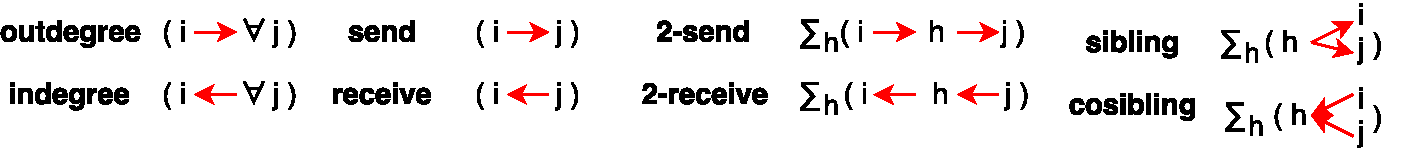
\includegraphics[height= 1.35cm, trim= 0cm 0cm 14cm 0cm, clip=true]{plots/netstats.pdf} \vspace{-.3cm}
 	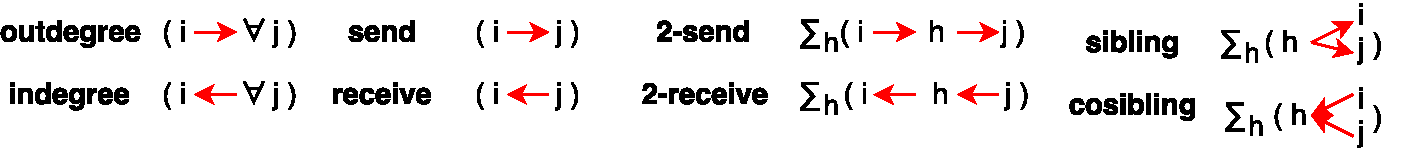
\includegraphics[height=1.35cm,, trim= 10cm 0cm 0cm 0cm, clip=true]{plots/netstats.pdf}
 	\caption{Eight dynamic network statistics used for the Dare County email network and Enron dataset.}
 	\label{fig:dynamic network statistics}	
 \end{figure}
 
Assuming that each network feature has potentially different effects within a number of time intervals (\textit{i.e.} recency effect), we partition the interval $[-\infty, t_d)$ into 4 sub-intervals with equal length in the log-scale, and focus on three time intervals prior to just after the email's timestamp: 3--16 days, 1--3 days, and
0--1 day. We disregard the time interval before 16 days, considering that the Dare County email network only spans 12 weeks in length. We then compute each of the network feature within each time interval to obtain a set of 24 dynamic network features $\boldsymbol{x}_{idjc}$, specific to author $i$, recipient $j$, email $d$, and interaction pattern $c$. Detailed mathematical formulations and corresponding interpretations of the network statistics are provided in Appendix C.

\subsection{Timestamp Specifications}\label{subsec:Timestamp Specifications}
Section \ref{subsubsec:Hypothetical Timestamps} presented a set of covariates $\boldsymbol{y}_{idjc}$ which are used to predict the timestamps of documents. Similarly as dynamic network features, we exemplify our choice of time-related features that are used to analyze the Dare County email network. First of all, we include the set of 24 dynamic network features $\boldsymbol{x}_{idjc}$ defined in Section \ref{subsec:Dynamic Network Statistics} as the component of $\boldsymbol{y}_{idjc}$, since ``who talked to whom, how often and recent, and about what" could play a important role in determing ``when to send" a document. Taking into account the fact that our data consists of government organizational emails as well as the exploratory results, we added two temporal features into $\boldsymbol{y}_{idjc}$ that stongly affects the timing of documents: the day of the week and time of the day when the previous document was sent. 

Moreover, our exploratory analysis revealed that the Dare County email network shows the best fitting when we specify lognormal distribution on the observed timestamps (\textit{i.e.} $\log(\tau_{a_dd}) \sim N(\mu_{a_d d}, V(\mu_{a_d d}) = \sigma^2_\tau))$, while we observed significant lack-of-fit for single parameter distributions such as Exponential distribution (\textit{i.e.} $\tau_{a_dd} \sim \mbox{Exp}(\mu_{a_d d}))$. Based on this result, we chose lognormal distribution. 

\section{Experiments}\label{sec:Experiments}
In this section, we conduct a set of posterior predictive experiments using the Dare County email network and the Enron dataset, to showcase the IPTM's predictive performance as compared to alternative modeling approaches.
\subsection{Tie Prediction}\label{subsec:Tie Prediction}
 For a randomly chosen document $d^* \in \{M, M+1,\ldots, D\}$, we fit the IPTM to the corpus consisting of the first $d = \{1,\hdots,d^*-1\}$ documents, then use the inferred posterior distributions to generate a distribution of predicted tie data ($a_{d^*}, \boldsymbol{r}_{d^*}, t_{d^*}$) conditional on the content in the document   $\boldsymbol{w}_{d^*}$, and compare the simulated ones to the observed data. We also compare the IPTM to the alternative model that is built upon two separate regression models for the recipients and timestamps, in order to test if the IPTM has any benefit over other existing models by jointly inferring the parameters that govern the generation of tie data---authors, recipients, and timestamps. Pseudocodes for generating predicted tie data using the IPTM and the regression model are demonstrated in Appendix D.
 
 For both data sets, the Dare County email network and Enron dataset, we randomly selected 200 documents from the later half of the corpus (\textit{i.e.} $M = \frac{D}{2}$) and generated 100 samples of predicted tie data for every document $d^*$. We ran the same predictive experiments with 21 unique combinations of the number of interaction patterns ($C = 1, 2, 3$) and the number of topics ($K = 2, 5, 10, 25, 50, 75, 100$) as a grid-search based hyperparameter selection process. We compare the predictions in terms of classification accuracy in predicting the authors and recipients, as well as prediction error in the timestamps. Figure \ref{fig:PPE} presents the $F_1$ scores on author predictions, multiclass version of the area under the ROC curve (AUC) measure \citep{hand2001simple} on reciptient predictions, and median absolute error (MAE) on timestamp predictions for each document we predicted, all averaged over the entire samples. The outcomes demonstrate the ability IPTM in predicting the author, recipient, and timetsamps of email. \textbf{Further comments after we conduct experiment again.}
 \begin{figure}[h]
 	\centering
	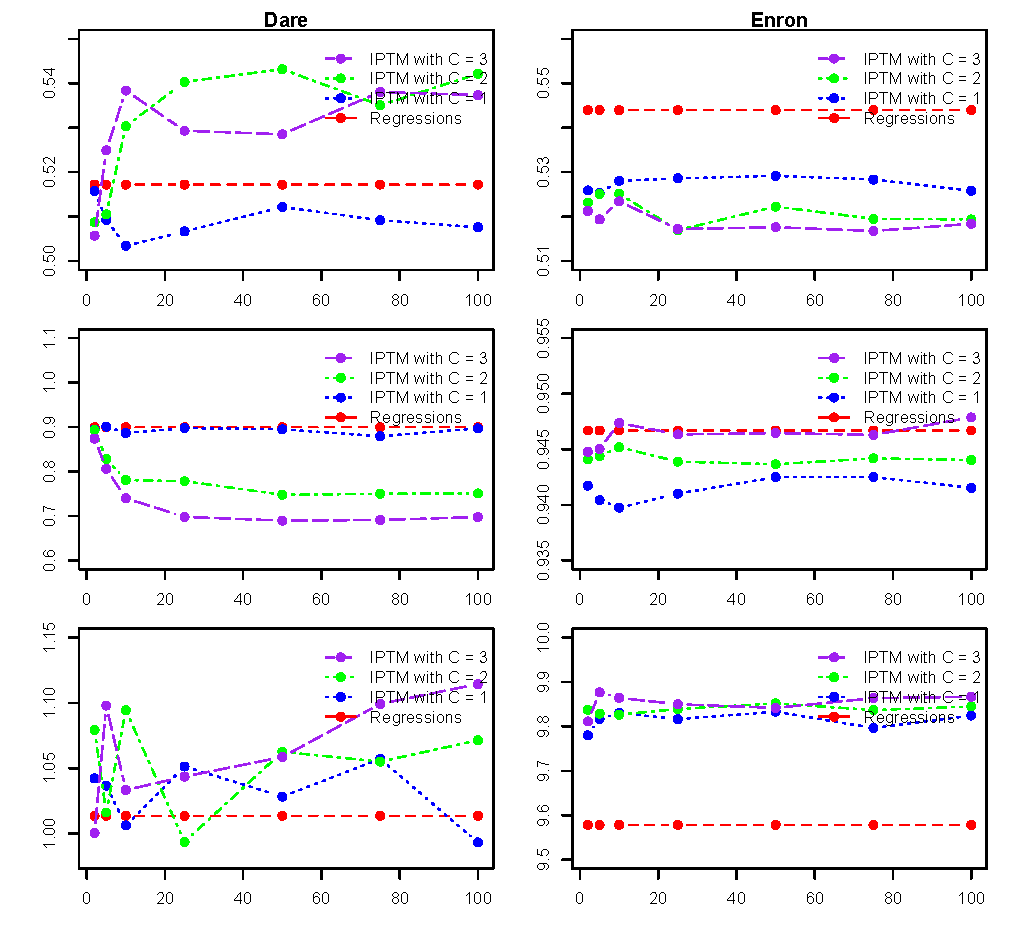
\includegraphics[width=0.49\textwidth, trim= 0.7cm 0cm 0cm 0cm, clip=true]{plots/PPE.pdf}  
 	\caption{Average AUC, F1 score, MAE: (\textit{top}) Dare County email network. (\textit{bottom}) Enron dataset.}
 	 	\label{fig:PPE}	
 	 \end{figure}
\subsection{Topic Coherence}\label{subsec:Topic Coherence}
Topic coherence metrics \cite{mimno2011optimizing} are often used to evaluate the semantic coherence in topic models. In order to test whether the IPTM's incorporation of network features improves the ability of modeling text, we compared the coherence of topics inferred using our model with the coherence of topics inferred using the latent dirichlet allocation (LDA). Instead of re-fit the data using standard LDA algorithms, we used the topic assignments from the IPTM with $C=1$, which simply makes the IPTM reduced to LDA in terms of topic assignments by unlinking the text and networks. For each model, we varied the number of topics from 1 to 100 and draw five samples from the joint posterior distribution over the latent variable. We evaluated the topics resulting from each sample and averaged over the five samples, where the results are shown in Figure \ref{fig:topic}. Combined with the results in Section \ref{subsec:Tie Prediction}, this result demonstrates that the IPTM can achieve good predictive performance while producing coherent topics. 
\begin{figure}[h]
	\centering
	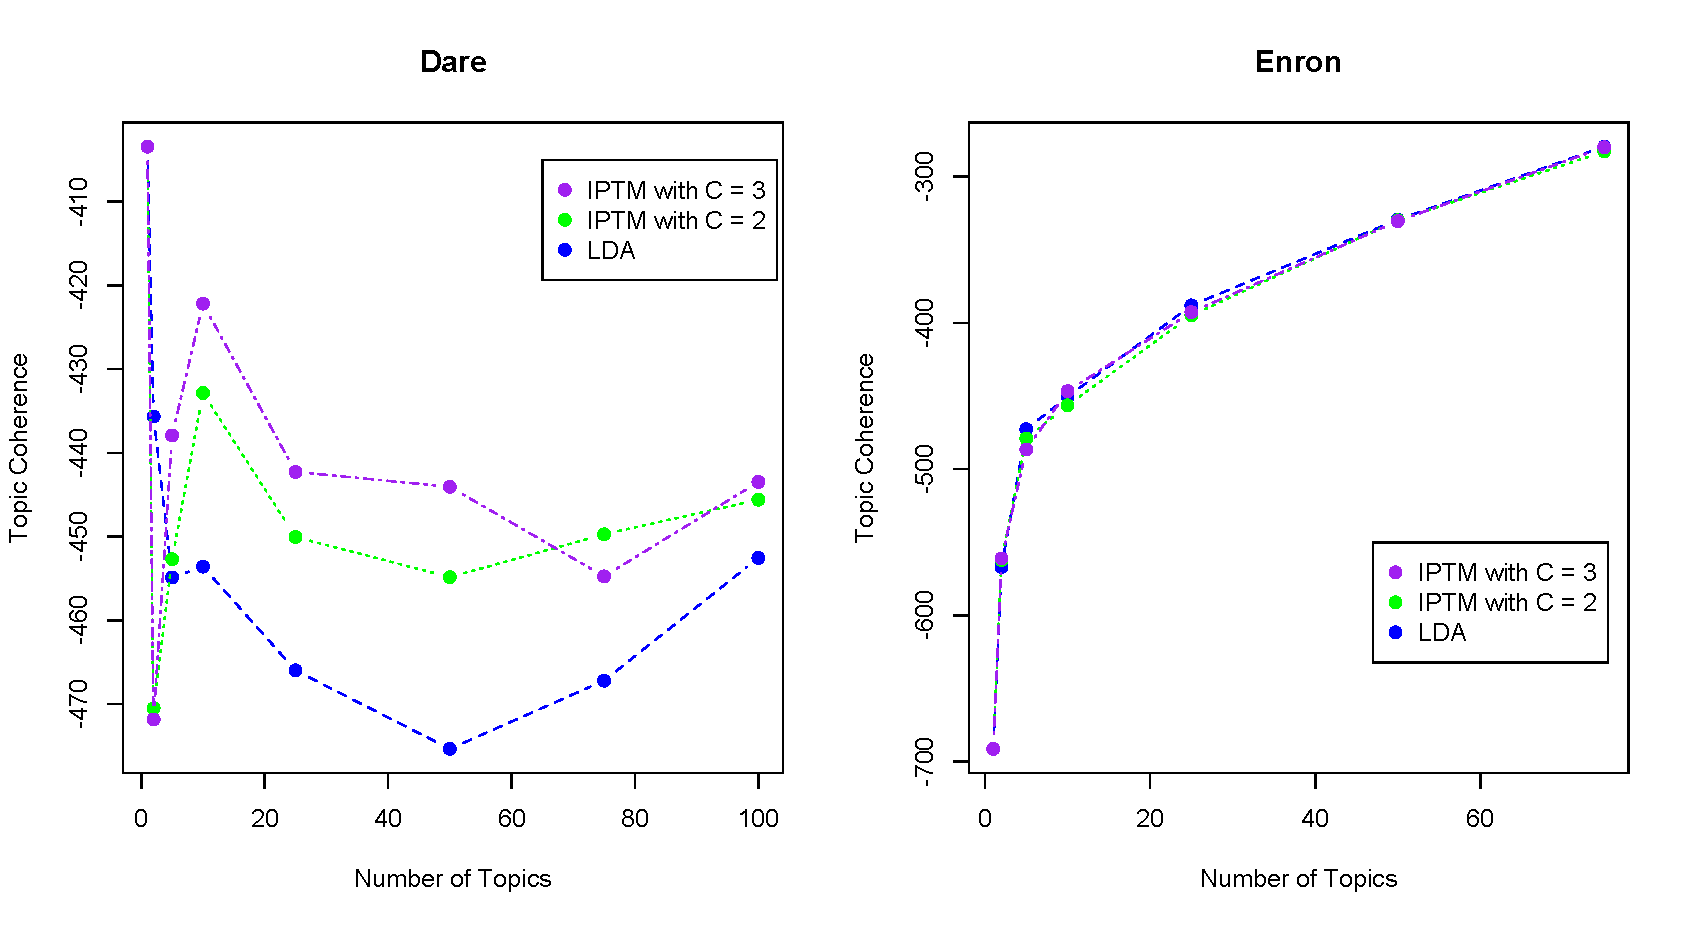
\includegraphics[width = 0.47\textwidth]{plots/topic_coherence.pdf}
	\caption{Average topic coherence scores: (\textit{left}) Dare County email network. (\textit{right}) Enron dataset.}
	\label{fig:topic}
	\end{figure}
\subsection{Posterior Predictive Checks}
We finally perform posterior predictive checks \cite{rubin1984bayesianly} in order to evaluate the appropriateness of the model specification for the Dare County email network. Formally, we generated entirely new data, by simulating $\{(a_{d}, \boldsymbol{r}_{d}, t_{d}, \boldsymbol{w}_{d})\}_{d=1}^D$ from the genenerative process in Section \ref{subsec:Content generating process} and \ref{subsec:Tie generating process}, conditional upon a set of inferred parameter values from the inference in Section \ref{sec:Inference}. For the test of goodness-of-fit in terms of network dynamics, we defined multiple network statistics that summarize meaningful aspects of the Dare County email networks: indegree distribution for author activities, outdegree distribution for recipient activities, recipient size distribution, document time-increment distributions, the edgewise shared partner distribution, and the geodesic distance distribution. For content-wise goodness-of-fit, we employed mutual information (MI) in \cite{mimno2011bayesian}, which is often used to evaluate ``bag of words" model assumptions. We then generated 1,000 synthetic networks and texts from the posterior predictive distribution implied by the IPTM and Dare County email network.
We applied each discrepancy function to each synthetic network to yield the distributions over the values of the six network statistics and MI. If the model is appropriate, the observed data should not be an outlier with respect to distributions of new data drawn from the posterior predictive distribution. 

Figure \ref{fig:PPC} illustrates the result of posterior predictive checks, showing IPTM's goodness of fit for Dare County data. The results reveal that IPTM captures some important work features of the data, including spreadness and transitivity. \textbf{Further comments after we conduct PPC again.}
	\begin{figure}[h]
		\centering
		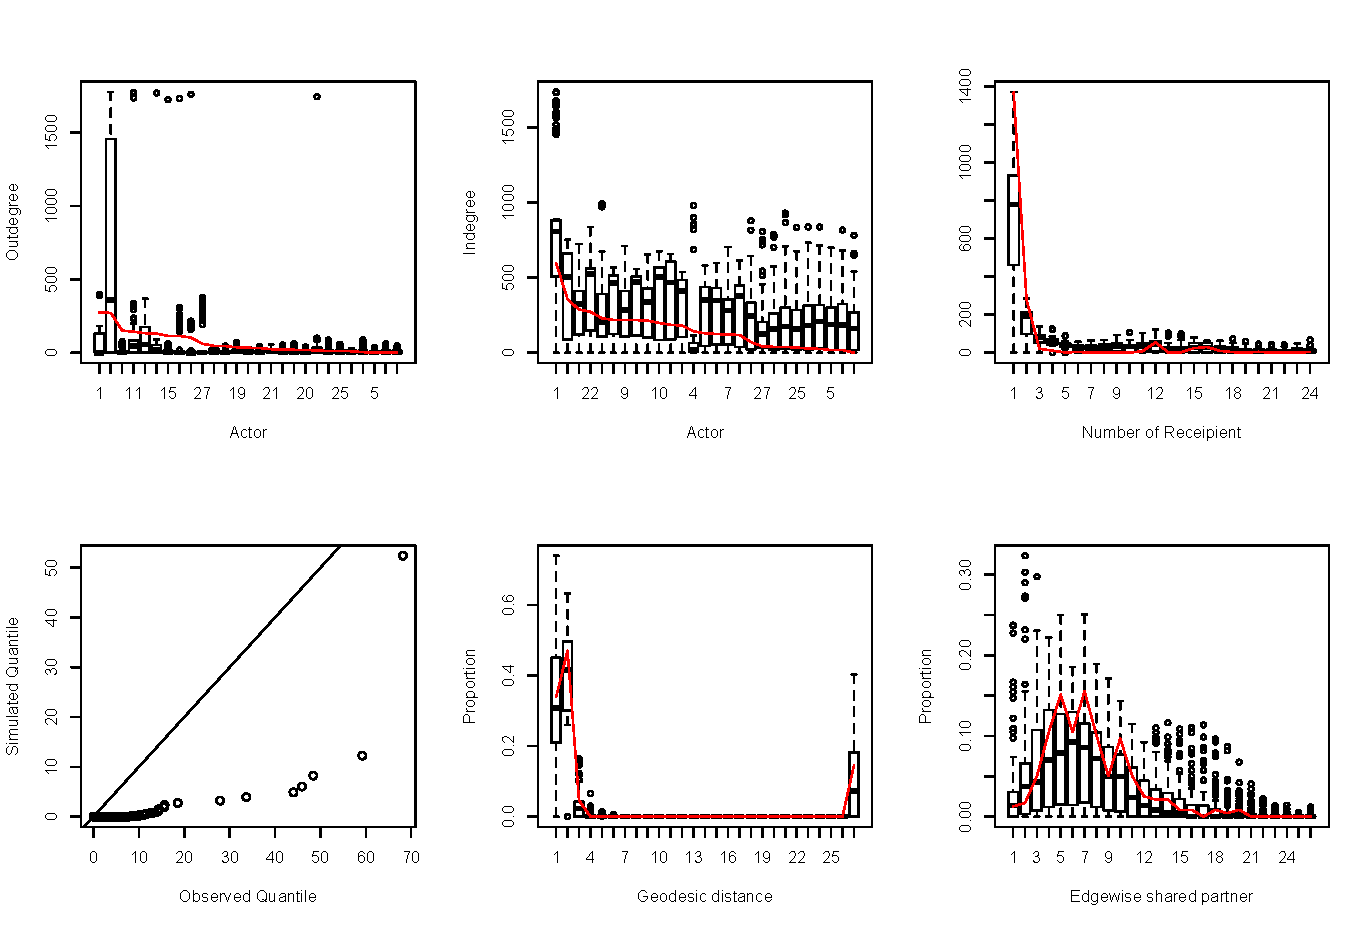
\includegraphics[width = 0.47\textwidth]{plots/PPC_plot.pdf}
		\caption{Posterior predictive checks for the Dare County email network: (a) outdegree, (b) indegree, (c) recipient size, (d) QQplot of time-increments, (e) geodesic distance, and (f) edgewise shared partners.}
		\label{fig:PPC}
	\end{figure}
\section{Analysis}\label{sec:Analysis}
In order to demonstrate our model's novel ability to identify interaction-pattern-specific communications that exist in both the content and relational structure, we performed an exploratory analysis on the interaction patterns inferred from the Dare County email network using the IPTM. Our main focus was to test three hypotheses: 1) personal or social topics (if any) would exhibit strong reciprocity and transitivity in tie formation, 2) topics about dissemination of information would be characterized by a lack of reciprocity, and 3) topics about Hurricane Sandy would exhibit a very different
interaction pattern from the normal day-to-day conversations.
\subsection{Topic Assignments}\label{subsec:Topic Assignments}
\begin{center}
	\scalebox{0.75}{	 
		\begin{tabular}{ |c|c|c|c|c|}
			\hline
			\textbf{23}&   \textbf{18} &\textbf{11} &\textbf{20} &\textbf{8}  \\ \hline\hline
			
			change & will &  \cellcolor{blue!25} sandy & time & services\\
			order & \cellcolor{blue!25}  winds &  munis & hours & public \\
			manager &  location & \cellcolor{blue!25} hurricane& monday & white\\
			\cellcolor{blue!25} storm & \cellcolor{blue!25} beach &  position & leave & director \\
			\cellcolor{blue!25}emergency &  \cellcolor{blue!25} hydrant & monday &employees & fyi\\
			\cellcolor{blue!25} coastal & \cellcolor{blue!25} water & point & timesheets &tim \\
			statute & relocation &  power& \cellcolor{blue!25} storm & \cellcolor{blue!25} update \\
			\cellcolor{blue!25}evacuation & mirlo & update & employee & \cellcolor{blue!25} status\\
			\cellcolor{blue!25} track &  road & \cellcolor{blue!25} storm& tomorrow &board \\
			couple & high & hey & work & approval\\
			\hline
		\end{tabular}}
	\end{center}
	\begin{center}
		\scalebox{0.7}{	 	\begin{tabular}{ |c|c|c|c|c|}
				\hline
				\textbf{21} & \textbf{12} &\textbf{14} &\textbf{4} &\textbf{10} \\ \hline\hline
				library & marshall & will&board & survey\\
				best & collins &center&meeting & request\\
				start & drive &day& property &call \\
				web & manteo & office&planning & sure\\
				place & phone & great&will & people\\
				visit &box & manager&notice &emergency \\
				albermarle & fax &assistance&  january & thought\\
				east & resources & problem& review & seafood\\
				regional & director & lot&commissioners & mail\\
				system & human & call&list & grant\\
				\hline
			\end{tabular}}
		\end{center}
		
\subsection{Interaction Pattern Coefficients}\label{subsec:Interaction Pattern Coefficients}
\begin{figure}[h]
	\centering
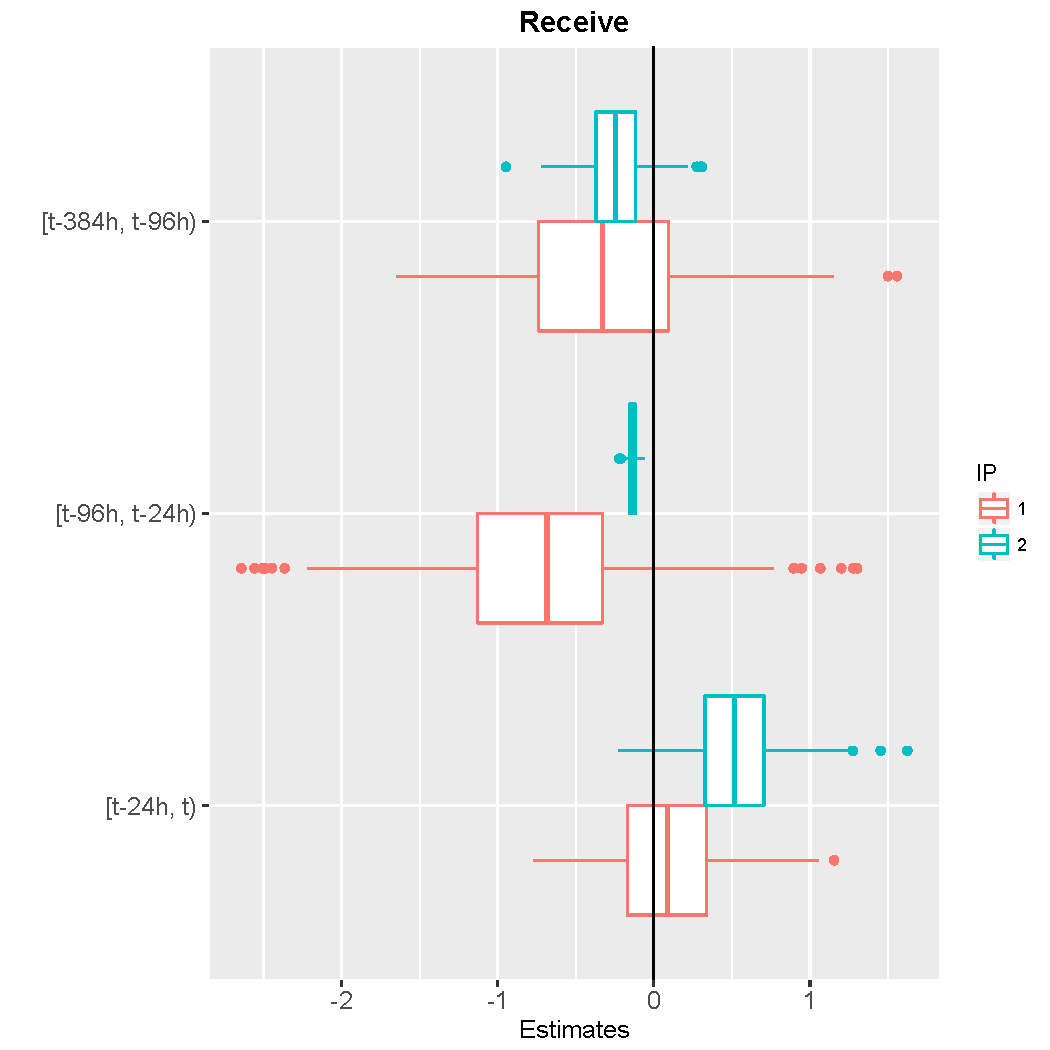
\includegraphics[width=.235\textwidth]{plots/receive.pdf} 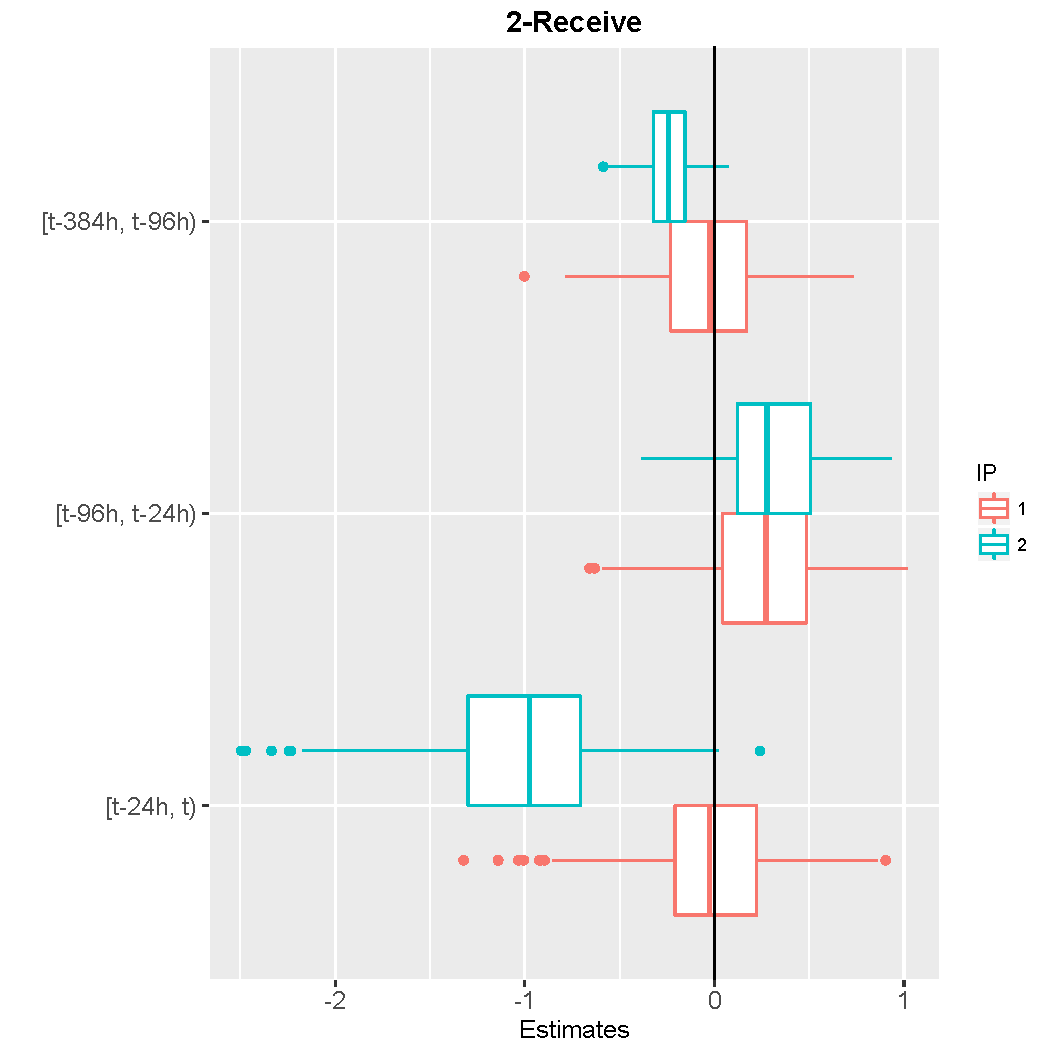
\includegraphics[width=.235\textwidth]{plots/2receive.pdf}
	\caption{95\% credible intervals of the posterior estimates of $\{\boldsymbol{b}_c\}_{c=1}^C$ using Dare County data: (\textit{left}) Recieve. (\textit{right}) 2-Recieve. }
	\label{fig:b}
\end{figure}
\section{Conclusions}\label{sec:Conclusions}
The IPTM is, to our knowledge, the first model to be capable of jointly modeling the author, recipients, timestamps and contents in time stamped text-valued networks. The IPTM incorporates innovative components, including the modeling of multicast tie formation and the conditioning of ERGM style network generative features on topic-based content. The application to North Carolina county government email data demonstrates, among other capabilities, the effectiveness at the IPTM in separating out both the content and relational structure underlying the normal day-to-day function of an organization and the management of a highly time-sensitive event---Hurricane Sandy. The IPTM is applicable to a variety of networks in which ties are attributed with textual documents. These include, for example, economic sanctions sent between countries and legislation attributed with sponsors and co-sponsors. 
\subsubsection*{Acknowledgements}
This work was supported in part by the University of Massachusetts Amherst Center for Intelligent Information Retrieval and in part by National Science Foundation grants DGE-1144860, SES-1619644, and CISE-1320219. Any opinions, findings, and conclusions or recommendations are those of the authors and do not necessarily reflect those of the sponsors.
\bibliographystyle{apalike}
\bibliography{IPTM}
\newpage
\appendix
\section*{Appendix}
\renewcommand{\thesubsection}{\Alph{subsection}}
  	 \subsection{Normalizing constant of Gibbs measure}\label{subsec: non-empty Gibbs measure}
  	 In Section \ref{subsubsec:Hypothetical Recipients}, we define the non-empty Gibbs measure such that the probability of author $i$ selecting the binary recipient vector $\boldsymbol{u}_{id}$ is given by
  	 \begin{equation*} 
  	 \footnotesize
  	 \begin{aligned}
  	& P(\boldsymbol{u}_{id}| \delta, \boldsymbol{\lambda}_{id} ) \\&= \frac{1}{Z(\delta,\boldsymbol{\lambda}_{id})} \exp\Big\{ \mbox{log}\Big(\text{I}(\lVert \boldsymbol{u}_{id} \rVert_1 > 0)\Big) + \sum_{j \neq i} \Big(\delta+\mbox{log}(\lambda_{idj})\Big)u_{idj} \Big\},
  	 \end{aligned}
  	 \end{equation*}
  	 where $Z(\delta,\boldsymbol{\lambda}_{id})$ is the normalizing constant omited in the main paper.
  	 To use this distribution efficiently, we derive a closed-form expression for $Z(\delta,\boldsymbol{\lambda}_{id})$ that does not require brute-force summation over the support of $\boldsymbol{u}_{id}$ (\textit{i.e.} $\forall \boldsymbol{u}_{id} \in [0,1]^A$). We recognize that if $\boldsymbol{u}_{id}$ were drawn via independent Bernoulli distributions in which $P({u}_{idj}=1|\delta, \boldsymbol{\lambda}_{id})$ was given by logit$(\delta+\log(\lambda_{idj}))$, then \begin{equation*}
  	 P(\boldsymbol{u}_{id}|\delta, \boldsymbol{\lambda}_{id}) \propto \exp\Big\{\sum_{j \neq i } \Big(\delta+\log(\lambda_{idj})\Big)u_{idj}\Big\}.  	 
  	 \end{equation*}
  	 This is straightforward to verify by looking at 
  	 \begin{equation*}
  	 \begin{aligned}
  &P(u_{idj}=1|\boldsymbol{u}_{id[-j]}, \delta, \boldsymbol{\lambda}_{id})
  	 =\frac{ \exp{\Big(\delta+\log(\lambda_{idj})\Big)}}{\exp{\Big(\delta+\log(\lambda_{idj})\Big)} + 1}.\end{aligned}\end{equation*}
  	 We denote the logistic-Bernoulli normalizing constant as $Z^{l}(\delta,\boldsymbol{\lambda}_{id})$, which is defined as 
  	 \begin{equation*}
  	 Z^{l}(\delta,\boldsymbol{\lambda}_{id})=\sum_{\boldsymbol{u}_{id} \in [0,1]^{A}} \exp\Big\{\sum_{j\neq i} \Big(\delta+\log(\lambda_{idj})\Big)u_{idj}\Big\}.
  	 \end{equation*}
  	 
  	 Now, since 
  	 \begin{equation*}
  	 \begin{aligned}
  	 &\exp\Big\{ \mbox{log}\Big(\text{I}(\lVert \boldsymbol{u}_{id} \rVert_1 > 0)\Big) + \sum_{j \neq i} \Big(\delta+\mbox{log}(\lambda_{idj})\Big)u_{idj} \Big\}\\&= \exp\Big\{  \sum_{j \neq i} \Big(\delta+\mbox{log}(\lambda_{idj})\Big)u_{idj} \Big\},
\end{aligned}
 	 \end{equation*}
 	  except when $\lVert \boldsymbol{u}_{id} \rVert_1=0$, we note that 
  	 \begin{equation*}
  	 \begin{aligned}
  	 Z(\delta,\boldsymbol{\lambda}_{id})& = Z^{l}(\delta,\boldsymbol{\lambda}_{id}) -  \exp\Big\{ \sum\limits_{\forall u_{idj}=0}\Big(\delta+\log(\lambda_{idj})\Big)u_{idj} \Big\}
  	 \\& = Z^{l}(\delta,\mbox{log}(\lambda_{i}^{(d)})) -  1.
  	 \end{aligned}
  	 \end{equation*}
  	 We can therefore derive a closed form expression for $Z(\delta,\boldsymbol{\lambda}_{id})$ via a closed form expression for $Z^{l}(\delta,\boldsymbol{\lambda}_{id})$. This can be done by looking at the probability of the zero vector under the logistic-Bernoulli model:
  	 \begin{equation*}
  	 \footnotesize
  	 \begin{aligned}
  	 &\frac{\exp\Big\{ \sum\limits_{\forall u_{idj}=0}\Big(\delta+\log(\lambda_{idj})\Big)u_{idj} \Big\}}{Z^{l}(\delta,\boldsymbol{\lambda}_{id})}\\&= \prod_{j \neq i}   \Big(1-\frac{ \exp{\Big(\delta+\log(\lambda_{idj})\Big)}}{\exp{\Big(\delta+\log(\lambda_{idj})\Big)} + 1}\Big).
  	  \end{aligned}  
  	  \end{equation*}
  	  Then, we have 
  	    	 \begin{equation*}
  	    	 \begin{aligned}
  	& Z^{l}(\delta,\boldsymbol{\lambda}_{id}) &= \frac{1}{\prod\limits_{j \neq i}   \frac{ \exp\{-(\delta+\mbox{log}(\lambda_{idj}))\}}{\exp\{-(\delta+\mbox{log}(\lambda_{idj}))\} + 1}}.
  	 \end{aligned}  
  	 \end{equation*}
  	 The closed form expression for the normalizing constant under the non-empty Gibbs measure is  \begin{equation*}
  	 \begin{aligned}Z(\delta,\boldsymbol{\lambda}_{id}) = \prod_{j \neq i } \Big(\mbox{exp}\{\delta+\mbox{log}(\lambda_{idj})\} + 1\Big)-1.
  	 \end{aligned}  
  	 \end{equation*}
  	
  	 \subsection{Sampling Equations}\label{subsec:Sampling Equations}
  	   \subsubsection{Resampling Hypothetical Recipients} \label{subsec: Resampling Hypothetical Recipients}
  	   First of all, for each document $d=1,\ldots, D$, we sample the latent recipients for each author other than the observed one (\textit{i.e.} $i \neq a_d$). 
  	   
  	   For each latent author $i$, we are going to resample $u_{idj}$, which is the $j^{th}$ element of the binary vector $\boldsymbol{u}_{id}$, one at a time with random order. The full conditional probability of $u_{idj}$ is:
  	   \begin{equation*}
  	   \begin{aligned}
  	   & P(u_{idj}|\boldsymbol{u}_{id[-j]},  \boldsymbol{z}_d,\boldsymbol{l},\boldsymbol{b}, \boldsymbol{\eta}, \delta, \boldsymbol{w}_d, \boldsymbol{a}_d, \boldsymbol{r}_d, \boldsymbol{t}_d)
\\&\propto P(u_{idj}, \boldsymbol{u}_{id[-j]}, \boldsymbol{a}_d, \boldsymbol{r}_d, \boldsymbol{t}_d| \boldsymbol{z}_d,\boldsymbol{l},\boldsymbol{b}, \boldsymbol{\eta}, \delta)
  	   \\&\propto \prod_{i=1}^A p(u_{idj}, \boldsymbol{u}_{id[-j]}|\boldsymbol{z}_d,\boldsymbol{l}, \boldsymbol{b}, \delta)\times p(\tau_{a_d d}|\boldsymbol{z}_d,\boldsymbol{l}, \boldsymbol{\eta})\\&\quad\quad\quad \times \prod_{i\neq a_d} p(\tau_{id} >\tau_{a_d d}|\boldsymbol{z}_d,\boldsymbol{l}, \boldsymbol{\eta}) \\& 
  	   = \prod_{i=1}^A L_{gibbs}(u_{idj}, \boldsymbol{u}_{id[-j]}| \delta, \boldsymbol{\lambda}_{id} )\times \varphi_{\tau}\big(\tau_{a_d d}; \mu_{a_d d}, V(\mu_{a_d d})\big)\\&\quad\quad\quad \times  \prod_{i\neq a_d}\Big(1-\Phi_{\tau} \big(\tau_{a_d d}; \mu_{i d}, V(\mu_{i d})\big) \Big)
  	     	   \end{aligned}\label{eqn:latentreceiver}
  	   \end{equation*}
  	   where we replace typical use of $(-d)$ to $(<d)$ on the right hand side, due to the fact that $d^{(th)}$ document only depends on the past documents. The last line of Equation (\ref{eqn:latentreceiver}) is obtained by dropping the terms that do not include $J^{(d)}_{ij}$, such as the normalizing constant of Gibbs measure. 
  	   
  	   To be more specific, since ${J}^{(d)}_{ij}$ could be either 1 or 0, we divide into two cases as below:
  	   \begin{equation}
  	   \begin{aligned}
  	   &P(\mathcal{J}^{(d)}_{ij}=1| \mathcal{J}^{(d)}_{i\backslash j}, \mathcal{T}^{(d)}_{\mbox{a}, i}, i^{(d)}_{\mbox{o}}, J^{(d)}_{\mbox{o}}, t^{(d)}_{\mbox{o}}, \mathcal{I}^{(<d)}_{\mbox{o}}, \mathcal{J}^{(<d)}_{\mbox{o}}, \mathcal{T}^{(<d)}_{\mbox{o}}, \mathcal{Z}, \mathcal{C}, \mathcal{B}, \delta, \boldsymbol{\eta}, \sigma_T^2)\\& \propto \mbox{exp}\Big(\log(1) +\sum_{j \in \mathcal{A}_{\backslash i}} ( \delta+\mbox{log}(\lambda_{ij}^{(d)}))J_{i[+j]}^{(d)}\Big) \times\Big(1 - \Phi_l(\Delta T^{(d)}_{i_o^{(d)}J_o^{(d)}};\boldsymbol{\eta}^T\boldsymbol{y}^{(d)}_{iJ_{i[+j]}}, \sigma_T^2)\Big)
  	   \\& \propto \mbox{exp}\Big(\delta+\mbox{log}(\lambda_{ij}^{(d)})\Big)\times\Big( 1 - \Phi_l(\Delta T^{(d)}_{i_o^{(d)}J_o^{(d)}};\boldsymbol{\eta}^T\boldsymbol{y}^{(d)}_{iJ_{i[+j]}}, \sigma_T^2)\Big),
  	   \end{aligned}\label{eqn:Jij1}
  	   \end{equation}
  	   where $J^{(d)}_{i[+j]}$ meaning that the $j^{th}$ element of $J_{i}^{(d)}$ is fixed as 1 (thus making $\mbox{log}\big(\text{I}(\lVert J_{i}^{(d)} \rVert_1 > 0 )\big) = 0$ for sure). On the other hand, 
  	   \begin{equation}
  	   \begin{aligned}
  	   &P(\mathcal{J}^{(d)}_{ij}=0| \mathcal{J}^{(d)}_{i\backslash j}, \mathcal{T}^{(d)}_{\mbox{a}, i}, i^{(d)}_{\mbox{o}}, J^{(d)}_{\mbox{o}}, t^{(d)}_{\mbox{o}}, \mathcal{I}^{(<d)}_{\mbox{o}}, \mathcal{J}^{(<d)}_{\mbox{o}}, \mathcal{T}^{(<d)}_{\mbox{o}}, \mathcal{Z}, \mathcal{C}, \mathcal{B}, \delta, \boldsymbol{\eta}, \sigma_T^2)\\& \propto \mbox{exp}\Big(\mbox{log}\big(\text{I}( \lVert J_{i[-j]}^{(d)} \rVert_1> 0 )\big) + \sum_{j \in \mathcal{A}_{\backslash i}} (\delta+\mbox{log}(\lambda_{ij}^{(d)}))J_{i[-j]}^{(d)} \Big)\times \Big( 1 - \Phi_l(\Delta T^{(d)}_{i_o^{(d)}J_o^{(d)}};\boldsymbol{\eta}^T\boldsymbol{y}^{(d)}_{iJ_{i[-j]}}, \sigma_T^2)\Big)
  	   \\& \propto \mbox{exp}\Big(\mbox{log}\big(\text{I}( \lVert J_{i[-j]}^{(d)} \rVert_1 > 0 )\big) \Big)\times \Big(1 - \Phi_l(\Delta T^{(d)}_{i_o^{(d)}J_o^{(d)}};\boldsymbol{\eta}^T\boldsymbol{y}^{(d)}_{iJ_{i[-j]}}, \sigma_T^2)\Big),
  	   \end{aligned}\label{eqn:Jij0}
  	   \end{equation}
  	   where $J^{(d)}_{i[-j]}$ meaning similarly that the $j^{th}$ element of $J_{i}^{(d)}$ is fixed as 0. In this case, we cannot guarantee $\text{I}( \lVert J_{i[-j]}^{(d)} \rVert_1 > 0)=1$, so we have to leave the term. When it is zero, $\exp\{\mbox{log}\big(\text{I}( \lVert J_{i[-j]}^{(d)} \rVert_1 > 0 )\big)\} = 0$, thus we will sample 1 with probability 1. From this property of non-empty Gibbs measure, we prevent from the instances where the sender has no recipients to send the document. Now we can use multinomial sampling using the two probabilities, Equation (\ref{eqn:Jij1}) and Equation (\ref{eqn:Jij0}).
\end{document}
